\documentclass[12pt,a4paper]{report}

\usepackage[utf8]{inputenc} % pentru suport diacritice
\usepackage[romanian]{babel} % setări pentru limba română 
\usepackage{sansmathfonts}
\renewcommand\familydefault{\sfdefault} % sans serif
\DeclareFontSeriesDefault[sf]{bf}{bx}

\usepackage[margin=2.54cm]{geometry}	% dimensiuni pagină și margini
\usepackage{graphicx} % support the \includegraphics command and options
\usepackage{subcaption} % for subfigures

% formatting sections and subsections
\usepackage{textcase}
\usepackage[titletoc, title]{appendix}
\usepackage{titlesec}
\titleformat{\chapter}{\large\bfseries\MakeUppercase}{\thechapter}{2ex}{}[\vspace*{-1.5cm}]
\titleformat*{\section}{\large\bfseries}
\titleformat*{\subsection}{\large\bfseries}
\titleformat*{\subsubsection}{\large\bfseries}

\usepackage{chngcntr}
\counterwithout{figure}{chapter} % no chapter number in figure labels
\counterwithout{table}{chapter} % no chapter number in table labels
\counterwithout{equation}{chapter} % no chapter number in equation labels

\usepackage{booktabs} % for much better looking tables
\usepackage{url} % Useful for inserting web links nicely
\urlstyle{same}	% same font as regular text
\usepackage{scrextend} % for multiple footnote references
\usepackage{fnpct} % for multiple footnotes in the same place
\usepackage[bookmarks,unicode,hidelinks]{hyperref}

\usepackage{array} % for better arrays (eg matrices) in maths
\usepackage{paralist} % very flexible & customisable lists (eg. enumerate/itemize, etc.)
\usepackage{verbatim} % adds environment for commenting out blocks of text & for better verbatim
\usepackage{enumitem}
\setlist{noitemsep}

\usepackage{xurl} % for breaking long URLs
\usepackage{amsmath}
\usepackage{amssymb} % for math symbols

% for integrals
\newcommand*\diff{\mathop{}\!\mathrm{d}}
\newcommand*\Diff[1]{\mathop{}\!\mathrm{d^#1}}

\usepackage{amsthm}
\newtheorem{definition}{Definiția}

\captionsetup{font=small,width=0.8\textwidth}

%%% HEADERS & FOOTERS
\usepackage{fancyhdr}
\pagestyle{empty}
\renewcommand{\headrulewidth}{0pt}
\renewcommand{\footrulewidth}{0pt}
\lhead{}\chead{}\rhead{}
\lfoot{}\cfoot{\thepage}\rfoot{}



\newcommand{\HeaderLineSpace}{-0.25cm}
\newcommand{\UniTextRO}{UNIVERSITATEA POLITEHNICA DIN BUCUREȘTI \\[\HeaderLineSpace] 
FACULTATEA DE AUTOMATICĂ ȘI CALCULATOARE \\[\HeaderLineSpace]
DEPARTAMENTUL DE CALCULATOARE\\}
\newcommand{\DiplomaRO}{PROIECT DE DIPLOMĂ}
\newcommand{\AdvisorRO}{Coordonator științific:}
\newcommand{\BucRO}{BUCUREȘTI}

\newcommand{\UniTextEN}{UNIVERSITY POLITEHNICA OF BUCHAREST \\[\HeaderLineSpace]
FACULTY OF AUTOMATIC CONTROL AND COMPUTERS \\[\HeaderLineSpace]
COMPUTER SCIENCE AND ENGINEERING DEPARTMENT\\}
\newcommand{\DiplomaEN}{DIPLOMA PROJECT}
\newcommand{\AdvisorEN}{Thesis advisor:}
\newcommand{\BucEN}{BUCHAREST}

\newcommand{\frontPage}[6]{
\begin{titlepage}
\begin{center}
{\Large #1}  % header (university, faculty, department)
\vspace{50pt}
\begin{tabular}{p{6cm}p{4cm}}
\includegraphics[scale=0.8]{pics/upb-logo.jpg} &
	\includegraphics[scale=0.5,trim={14cm 11cm 2cm 5cm},clip=true]{pics/cs-logo.pdf}
\end{tabular}

\vspace{105pt}
{\Huge #2}\\                           % diploma project text
\vspace{40pt}
{\Large #3}\\ \vspace{0pt}  % project title
{\Large #4}\\                          % project subtitle
\vspace{40pt}
{\LARGE \Name}\\                   % student name
\end{center}
\vspace{60pt}
\begin{tabular*}{\textwidth}{@{\extracolsep{\fill}}p{6cm}r}
&{\large\textbf{#5}}\vspace{10pt}\\      % scientific advisor
&{\large \Advisor}                                    % advisor name
\end{tabular*}
\vspace{20pt}
\begin{center}
{\large\textbf{#6}}\\                                % bucharest
\vspace{0pt}
{\normalsize \Year}
\end{center}
\end{titlepage}
}

\newcommand{\frontPageRO}{\frontPage{\UniTextRO}{\DiplomaRO}{\ProjectTitleRO}{\ProjectSubtitleRO}{\AdvisorRO}{\BucRO}}
\newcommand{\frontPageEN}{\frontPage{\UniTextEN}{\DiplomaEN}{\ProjectTitleEN}{\ProjectSubtitleEN}{\AdvisorEN}{\BucEN}}

\linespread{1.15}
\setlength\parindent{0pt}
\setlength\parskip{.28cm}

%% Abstract macro
\newcommand{\AbstractPage}{
\begin{titlepage}
\textbf{\large SINOPSIS}\par
\AbstractRO\par\vfill
\textbf{\large ABSTRACT}\par
\AbstractEN \vfill
\end{titlepage}
}

%% Thank you macro
\newcommand{\ThanksPage}{
\begin{titlepage}
{\noindent \large\textbf{MULȚUMIRI}}\\
\Thanks
\end{titlepage}
}



%%%%%%%%%%%%%%%%%%%%%%%%%%%%%%%%%%%%%%%%%%%%%%%%%%   
%%
%%          End of template definitions
%%   
%%%%%%%%%%%%%%%%%%%%%%%%%%%%%%%%%%%%%%%%%%%%%%%%%%


%%% Puteți elimina aceste linii din lucrare, servesc numai pentru template.
\newcommand{\worktype}[1]{[\textit{#1}] }
\newcommand{\dezvoltare}{\worktype{Dezvoltare de produs}}
\newcommand{\cercetare}{\worktype{Cercetare}}
\newcommand{\ambele}{\worktype{Ambele}}
%%%


%%
%%   Campurile de mai jos trebuie modificate de autor. Modificati doar continutul, nu si numele fiecarei definitii
%%
\newcommand{\ProjectTitleRO}{Implementarea algoritmului Ray Tracing}
\newcommand{\ProjectSubtitleRO}{folosind arhitectura DirectX Raytracing}
\newcommand{\ProjectTitleEN}{Implementation of the Ray Tracing algorithm}
\newcommand{\ProjectSubtitleEN}{using the DirectX Raytracing architecture}
\newcommand{\Name}{Alex-Andrei Cioc}
\newcommand{\Advisor}{Conf. Dr. Ing. Victor Asavei}
\newcommand{\Year}{2024}

% Setări document
\title{Proiect de diplomă}
\author{\Name}
\date{\Year}

%%
%%   Campurile aferente rezumatului
%%
\newcommand{\AbstractRO}{
Algoritmul Ray Tracing este o tehnică de randare a imaginilor care simulează
propagarea și comportamentul razelor de lumină într-o scenă tridimensională. Acesta
este adesea folosit în industria cinematografică pentru a obține imagini fotorealiste.
Până de curând, natura computațională intensivă a acestui algoritm a limitat utilizarea
sa în aplicații interactive, precum jocurile video. Totuși, cu avansul tehnologiei,
utilizarea acestuia a devenit tot mai accesibilă și pentru
aceste aplicații. Suport hardware pentru Ray Tracing în contextul consumatorilor a fost
introdus de NVIDIA în 2018, prin intermediul arhitecturii Turing\footnote{\label{turing}\url{https://images.nvidia.com/aem-dam/en-zz/Solutions/design-visualization/technologies/turing-architecture/NVIDIA-Turing-Architecture-Whitepaper.pdf}. Accesat 10.06.2024.}.
Tot în același an, Microsoft a anunțat DirectX Raytracing\footnote{\label{dxr}\url{https://devblogs.microsoft.com/directx/announcing-microsoft-directx-raytracing/}. Accesat 10.06.2024.} (DXR),
o extensie a API-ului DirectX 12 care permite programatorilor să folosească
Ray Tracing în aplicațiile lor, utilizând hardware-ul compatibil.

Lucrarea de față își propune să studieze și să implementeze
algoritmul Ray Tracing pe un sistem de calcul modern, folosind accelerarea hardware
oferită de arhitectura DirectX Raytracing. Acest algoritm va fi folosit pentru
randarea iluminării unor scene arbitrare, în timp real, oferind o reprezentare fotorealistică a acestora.
În cadrul lucrării se va realiza o analiză a performanțelor implementării curente,
atât a fidelității imaginilor generate, cât și a eficienței spațio-temporale a implementării.
Se vor explora și posibilitățile de optimizare a algoritmului, precum și
modul în care acestea pot fi folosite pentru a îmbunătăți performanțele sistemului.
}

\newcommand{\AbstractEN}{The Ray Tracing algorithm is an image rendering technique that simulates
the propagation and behavior of light rays in a three-dimensional scene. It is
often used in the film industry to achieve photorealistic images.
Until recently, the computationally intensive nature of this algorithm has limited its use
in interactive applications, such as video games. However, with technological advances,
its use has become increasingly accessible for
these applications as well. Hardware support for Ray Tracing in the consumer context was
introduced by NVIDIA in 2018, through the Turing\footref{turing} architecture.
In the same year, Microsoft announced DirectX Raytracing\footref{dxr} (DXR),
an extension of the DirectX 12 API that allows programmers to use
Ray Tracing in their applications, using compatible hardware.

This paper aims to study and implement
the Ray Tracing algorithm on a modern computing system, using the hardware acceleration
provided by the DirectX Raytracing architecture. This algorithm will be used for
rendering the lighting of arbitrary scenes, in real-time, providing a photorealistic representation of them.
The paper will perform an analysis of the current implementation's performance,
both in terms of the fidelity of the generated images and the spatio-temporal efficiency of the implementation.
It will also explore the possibilities for optimizing the algorithm, as well as
how these can be used to improve the system's performance.}

%%
%%   Campurile aferente paginii de multumiri
%%
\newcommand{\Thanks}{Adresez mulțumiri coordonatorului meu de proiect, Conf. Dr. Ing. Victor Asavei, pentru îndrumarea
și sprijinul acordat pe parcursul realizării acestei lucrări, dar și pentru
inspirația și motivația oferită în cadrul cursurilor de Elemente de Grafică pe Calculator.
De asemenea, mulțumesc familiei și prietenilor pentru susținere și încurajare.}

\numberwithin{equation}{section} % for equation numbering

\begin{document}

\frontPageRO
\frontPageEN

\begingroup
\linespread{1}
\tableofcontents
\endgroup

\AbstractPage

% poate fi comentata sau stearsa
\ThanksPage


% Textul licentei incepe de aici 



\chapter{Introducere}\pagestyle{fancy}
% * <marios.choudary@gmail.com> 2018-02-28T11:38:18.106Z:
% 
% > INTRODUCERE
% Am scos de aici referintele la font pentru a nu mai fi dependenti de Calibri. Personal, nici nu sunt sigur ca ajuta prea mult aceasta recomandare si mi se pare bun font-ul default din Latex (Computer Modern). Daca sunteti de-acord, va rog sa stergeti liniile comentate de mai jos, precum si cele referitoare la fontul Calibri din restul documentului.
% 
% ^.


\section{Context}
Industria jocurilor video este una dintre cele mai mari și mai profitabile industrii
de divertisment din lume. În 2021, piața jocurilor video era evaluată la aproximativ
202.64 miliarde de dolari și este estimat să se extindă la o rată anuală compusă de creștere de 10.2\%
în perioada 2022-2030\footnote{\url{https://www.grandviewresearch.com/industry-analysis/gaming-industry}. Accesat 10.06.2024.}.
Această industrie este alimentată de cererea pentru experiențe interactive și captivante,
care să ofere o experiență de joc cât mai realistă și cât mai imersivă. Toate studio-urile
de dezvoltare de jocuri video AAA (i.e., jocuri cu bugete mari și echipe de dezvoltare
extinse) investesc resurse semnificative în dezvoltarea de tehnologii care să le permită
să creeze jocuri cu grafică de înaltă calitate. Aceste tehnologii includ motoare grafice
puternice, care să permită randarea unor scene complexe, cu iluminare realistă și efecte
speciale impresionante. Multe studio-uri folosesc propriile motoare dezvoltate
in-house (e.g., Frostbite de la EA, CryEngine de la Crytek, Anvil de la Ubisoft), dar
există și motoare comerciale, precum Unreal Engine și Unity. Aceste motoare oferă
un set de instrumente și funcționalități care permit dezvoltatorilor să creeze jocuri
video de înaltă calitate, fără a fi nevoie să dezvolte de la zero toate componentele
necesare. O componentă critică a acestor motoare este motorul grafic, care se ocupă
de randarea scenei jocului, de la geometria obiectelor până la iluminare și efecte
speciale. Astfel, programatorii, artiștii, animatorii și designerii de jocuri pot
să se concentreze pe crearea conținutului jocului, fără a fi nevoie să se ocupe
de detalii tehnice ale randării grafice.

\section{Problema}
Tehnica tradițională și cea mai răspândită de randare a imaginilor în jocurile video
este rasterizarea. Această tehnică se bazează pe proiecția obiectelor 3D pe un plan
bidimensional, folosind o serie de algoritmi și tehnici pentru a simula iluminarea și
efectele speciale. Rasterizarea este o tehnică eficientă și rapidă, care permite
randarea unui număr mare de obiecte în timp real, dar are și limitări. Una dintre
cele mai mari limitări ale rasterizării este incapacitatea de a simula iluminarea
globală, care este esențială pentru obținerea unor imagini fotorealiste. De asemenea,
reflexiile și refracțiile pot fi doar aproximate, de exemplu prin tehnici de cubemapping
sau screen-space reflections. Aceste tehnici sunt eficiente, dar nu oferă rezultate
realistice, iar în multe cazuri pot fi observate artefacte vizuale care afectează
calitatea imaginii.

În continuare se evidențiază aceste limitări (care nu sunt deloc exhaustive) ale
rasterizării, prin comparație cu tehnica de Ray Tracing (așa numita \textit{RTX} în
jocurile sponsorizate de Nvidia).
Comparând Figurile~\ref{fig:ssr-good} și~\ref{fig:ssr-bad}, se observă neajunsul
reflexiilor în screen space. Atâta timp cât obiectele reflectate se află în viewport,
reflexiile sunt corecte și realiste. Însă, dacă obiectele ies din viewport, reflexiile
se pierd, ceea ce duce la o imagine nerealistă. Un alt exemplu și mai elocvent este
ilustrat în Figura~\ref{fig:bf5-rtx}, unde imaginea randată cu Ray Tracing redă
reflexii ale exploziei care nu este vizibilă decât parțial în cadru.

\begin{figure}[ht]
	\centering
	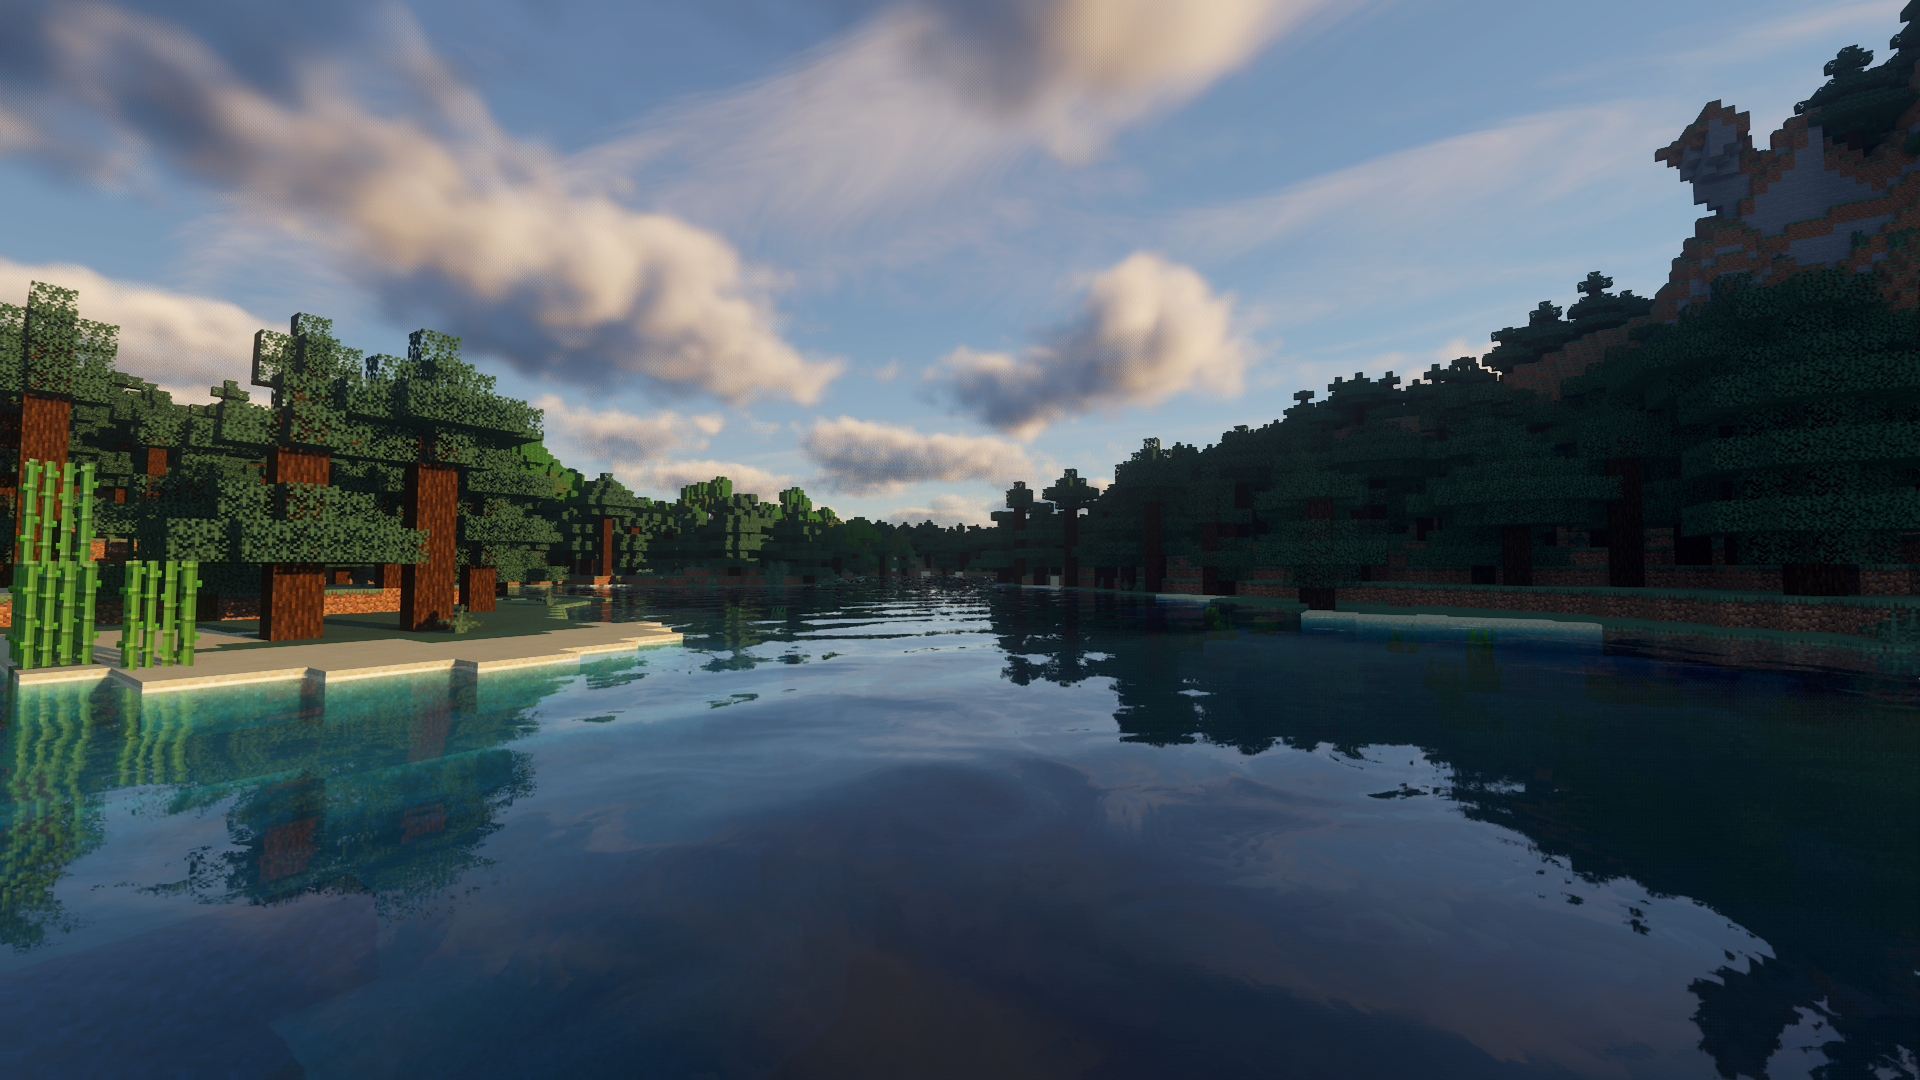
\includegraphics[width=0.8\textwidth]{pics/mc-ssr-good.png}
	\caption{Screen space reflections în Minecraft\protect\footnotemark}
	\label{fig:ssr-good}
\end{figure}
\footnotetext{\label{continuum}Shader folosit: \textcopyright \url{https://continuum.graphics/}. Accesat  10.06.2024.}

\begin{figure}[ht]
	\centering
	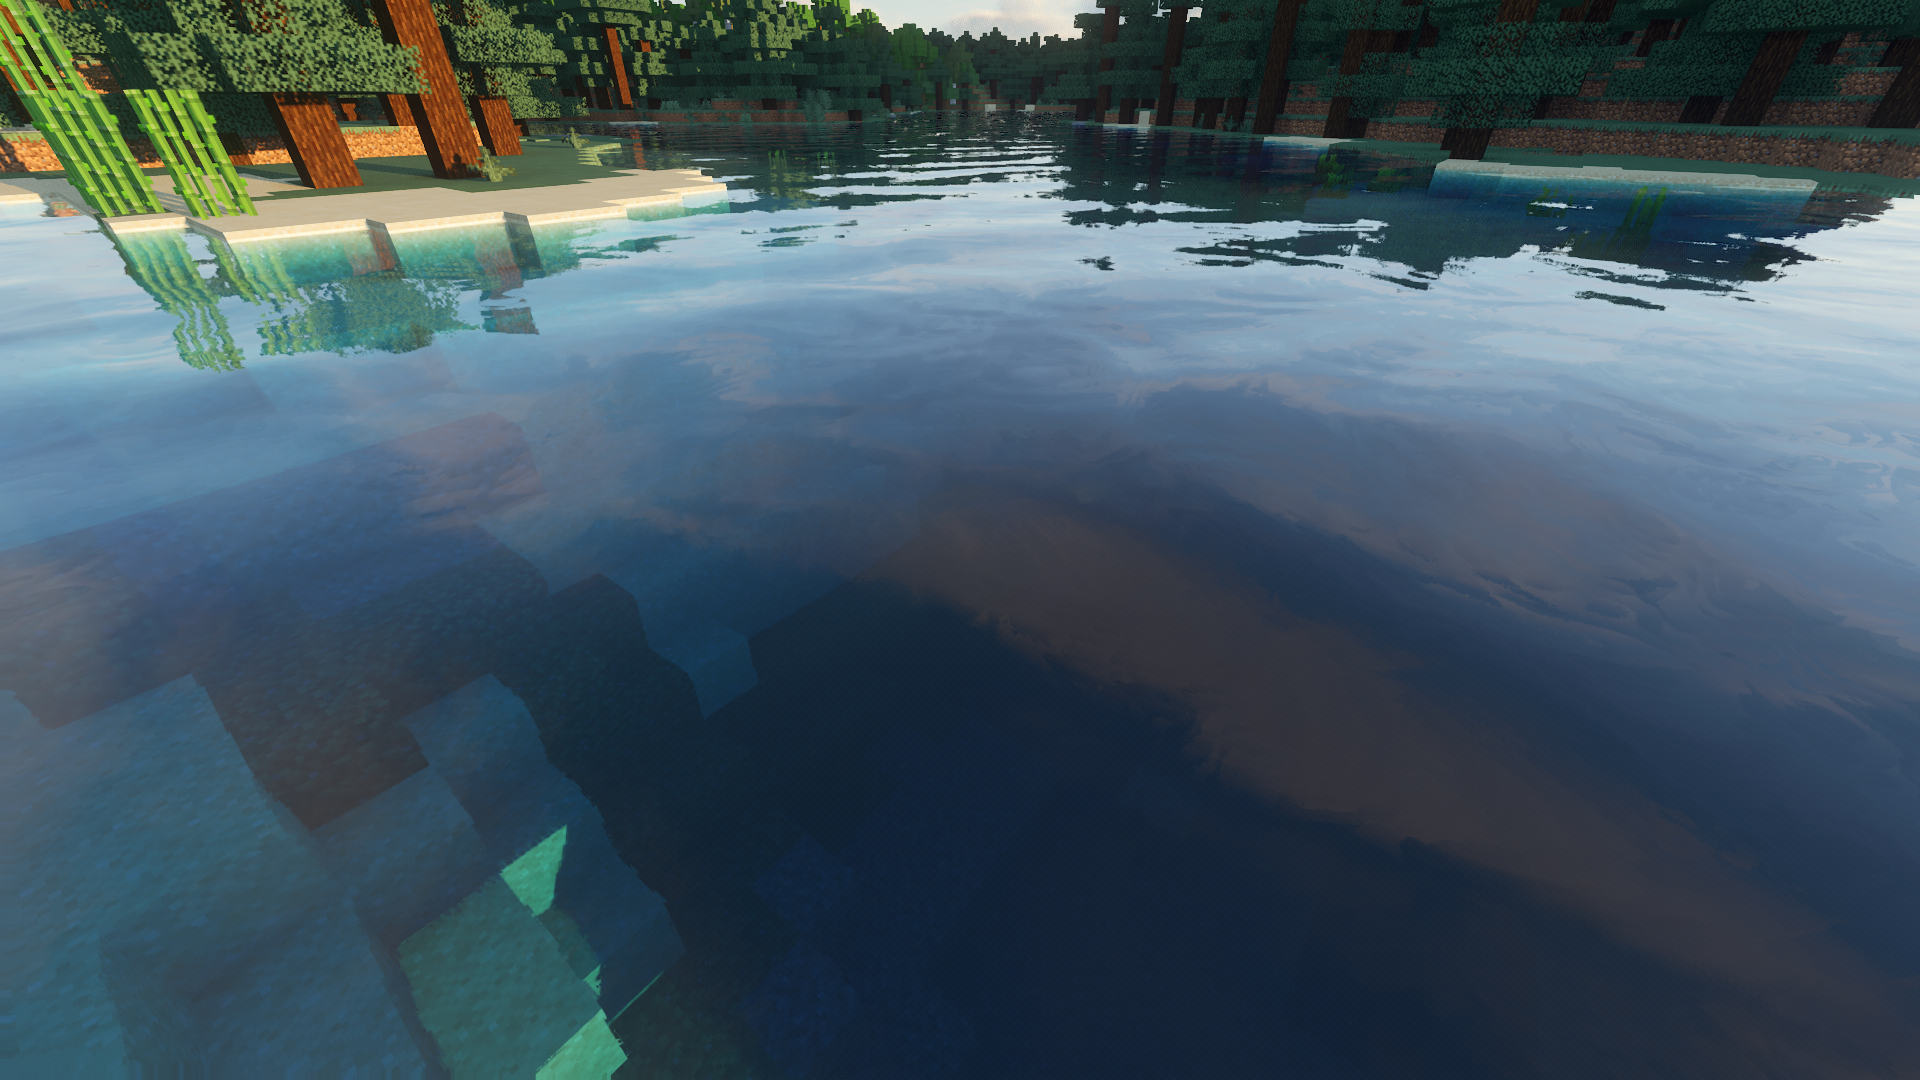
\includegraphics[width=0.8\textwidth]{pics/mc-ssr-bad.png}
	\caption{Artefacte vizuale în screen space reflections\protect\footref{continuum}. Se poate observa cum
		reflexiile se pierd dacă obiectele reflectate ies din viewport}
	\label{fig:ssr-bad}
\end{figure}

\begin{figure}[ht]
	\centering
	\includegraphics[width=0.8\textwidth]{pics/cornell-raster.jpg}
	\caption{Iluminarea globală este absentă în imaginea randată cu rasterizare\protect\footnotemark}
	\vspace{1cm}
	\label{fig:cornell-raster}
\end{figure}
\footnotetext{\textcopyright Nvidia Corporation: \url{https://blogs.nvidia.com/blog/geforce-rtx-real-time-ray-tracing/}. Accesat 10.06.2024.}

\begin{figure}[ht]
	\centering
	\begin{subfigure}[h]{0.45\linewidth}
		\centering
		\includegraphics[width=\linewidth]{pics/bf5-rtx-off.png}
		\caption{RTX off}
	\end{subfigure}
	\hfill
	\begin{subfigure}[h]{0.45\linewidth}
		\centering
		\includegraphics[width=\linewidth]{pics/bf5-rtx-on.png}
		\caption{RTX on}
	\end{subfigure}
	\caption{Comparație RTX on/off în Battlefield V\protect\footnotemark}
	\label{fig:bf5-rtx}
\end{figure}
\footnotetext{\textcopyright Nvidia Corporation: \url{https://www.youtube.com/watch?v=WoQr0k2IA9A}. Accesat 10.06.2024.}

Am văzut cum tehnica de Ray Tracing poate oferi rezultate mult mai realiste
decât rasterizarea, dar această tehnologie vine cu un cost.
Algoritmul Ray Tracing este computațional intensiv, deoarece necesită
calcularea intersecțiilor mai multor raze de lumină pentru fiecare pixel cu obiectele din scenă
și calcularea contribuției acestora la culoarea pixelului. Pentru a obține o imagine
de calitate, este nevoie de un număr mare de raze de lumină și tehnici de denoising,
ceea ce face ca algoritmul să fie greu de balansat între fidelitate și performanță.

\section{Obiective}

Scopul acestei lucrări este de a cerceta și implementa algoritmul Ray Tracing în
context de timp real și a evalua performanțele acestuia, prin comparație cu
implementări destinate producției cinematografice. Eforturile vor fi concentrate
pe implementarea unui motor grafic simplu, cu câteva funcționalități de bază:
\begin{itemize}
	\item Controale de cameră simple (mișcare, rotire)
	\item Randarea obiectelor definite ca mesh-uri triunghiulare
	\item Randarea obiectelor definite prin funcții implicite (e.g., sfere, planuri)
	\item Suport pentru materiale PBR (Physically Based Rendering)
	\item Suport pentru mai multe scene precum:
	      \begin{itemize}
		      \item Cornell Box\footnote{\url{https://www.graphics.cornell.edu/online/box/}. Accesat 19.06.2024.}
		      \item Demonstrație a suprafețelor implicite
		      \item Scenă de testare a materialelor PBR
	      \end{itemize}
	\item Meniu de configurare a mai multor parametri (e.g., pentru materiale,
	      configurarea algoritmului etc.),
\end{itemize}
precum și a unor efecte de iluminare care să ofere o imagine fotorealistică a scenei:
\begin{itemize}
	\item Iluminare globală
	\item Reflexii și refracții
	\item Umbre.
\end{itemize}
De asemenea, vom explora și implementa tehnici de optimizare a algoritmului propriu-zis,
pe care le vom evalua în contextul de performanță și fidelitate obținute.

În final, dorim să obținem o implementare eficientă, care să țintească un frametime de 16.6ms
(60 de cadre pe secundă) la o rezoluție Full HD (1920x1080), pentru hardware entry-level cu suport pentru
DirectX Raytracing (e.g., Nvidia GeForce RTX 2060).

\section{Soluția propusă}
Soluția propusă este un motor grafic simplu de utilizat. Din perspectiva utilizatorului,
acesta are un meniu din care poate configura diverși parametri ai algoritmului
de Ray Tracing, precum și ai scenei. Utilizatorul poate încărca scene predefinite
și poate interacționa cu acestea folosind controalele de cameră.

La nivel de bază, motorul grafic conține două implementări din clasa algoritmilor
de Ray Tracing. Prima este o versiune simplă a algoritmului original descris de
Whitted (1980)~\cite{Whitted}, peste care se aplică modelul clasic de iluminare
Phong (1975)~\cite{Phong}. Această implementare a fost adaptată din codul sursă
suport oferit de Microsoft\footnote{\url{https://github.com/microsoft/directx-graphics-samples/blob/master/Samples/Desktop/D3D12Raytracing/src/D3D12RaytracingProceduralGeometry/readme.md}. Accesat 19.06.2024.}.
A doua implementare este scrisă de la zero și folosește algoritmul de tip Monte Carlo
Path Tracing pentru a rezolva ecuația de iluminare globală propusă de Kajiya (1986)~\cite{Kajiya}.
Fără a intra în prea multe detalii tehnice (vezi secțiunea \ref{sec:stateoftheart}),
această ecuație descrie cantitatea de lumină emisă dintr-un punct de pe o suprafață,
de-a lungul unei direcții de vizualizare, dându-se o funcție de distribuție a luminii
și un BRDF (Bidirectional Reflectance Distribution Function) pentru materialul de pe
suprafață. Ecuația conține o integrală de suprafață (peste emisfera unitate), care
integrează contribuțiile din toate direcțiile. Pentru eficiență, această integrală
este eșantionată folosind tehnici de Importance Sampling, descrise în secțiunea \ref{sec:stateoftheart}.
Totuși, numărul de eșantioane per pixel rămâne în continuare foarte limitat, din
cauza bugetului de calcul (nu depășește 16 eșantioane per pixel). Pentru a reduce
în continuare varianța (manifestată prin zgomot în imaginea finală), se folosește
un algoritm de denoising în faza de post procesare. Mai multe detalii tehnice
despre implementare sunt prezentate în secțiunea \ref{sec:implementare}.

Algoritmul de Path Tracing folosește un sistem de materiale diferit de cel folosit
de algoritmul Whitted. Dacă acesta din urmă este limitat de modelul simplu de iluminare
Phong, Path Tracing folosește un model PBR (Physically Based Rendering) inspirat de
cel introdus de Burley în 2012~\cite{Disney}, pentru a fi folosit în producția filmelor
marca Walt Disney Animation Studios. Varianta implementată în această lucrare este
augmentată cu o componentă de transmisie, descrisă într-un curs organizat de Hill et al. la conferința SIGGRAPH din 2015~\cite{DisneyBSDF}.
Acest model este mult mai complex,
având la bază un BSDF (Bidirectional Scattering Distribution Function - oferă și
o componentă de transmisie a luminii prin materiale) care descrie cum un material
interacționează cu lumina incidentă. Fiind totuși folosit în producția cinematografică,
modelul se concentrează pe a avea o interfață cât mai intuitivă pentru artistul
grafic, deviând puțin de la un model fizic strict. Bazele teoretice și implementarea acestui model
PBR sunt descrise în secțiunile \ref{sec:stateoftheart} și \ref{sec:implementare}.

Pentru evaluare se folosesc 3 scene distincte. Prima este celebra Cornell Box
(o variantă se poate vedea în Figura~\ref{fig:cornell-raster}), care este folosită
pentru a evalua corectitudinea algoritmului de iluminare globală. Se va putea
face o comparație între cei doi algoritmi de Ray Tracing. Se va mai observa și
capabilitatea algoritmului de Path Tracing de a simula surse de lumină de tip
area light, care sunt dificil de modelat în algoritmul Whitted.
A doua scenă este un test al materialelor PBR, exclusivă pentru algoritmul de Path Tracing.
Aceasta conține mai multe sfere cu același material de bază, care diferă
printr-un singur parametru. Utilizatorul poate alege care să fie acest parametru
variabil și să seteze constante pentru restul parametrilor. Scena va fi folosită pentru
a evalua fidelitatea sistemului de materiale.
Ultima scenă testează performanțele de rulare a algoritmilor. Aceasta conține
mai multe obiecte simple, definite prin suprafețe implicite, dar și obiecte
complexe definite ca mesh-uri triunghiulare cu multe poligoane.

\section{Rezultatele obținute}

//TODO

Descriere pe scurt a rezultatelor obținute, eventual de ce acestea sunt importante față de alte soluții sau studii.

\section{Structura lucrării}

Vreau să încep prin a clarifica faptul că această lucrare nu își propune să introducă
noi metode sau concepte în domeniul graficii pe calculator. Scopul acesteia
este de a experimenta și de a înțelege mai bine tehnologiile existente, precum
și de a pune în practică teoria care stă la baza acestora. Lucrarea este structurată
într-o parte teoretică inițială, menită să familiarizeze cititorul printr-o introducere lină
în conceptele care stau la baza algoritmului de Path Tracing, și o parte practică,
care se concentrează pe utilizarea API-ului DirectX12 pentru a implementa algoritmul
cu accelerare hardware. Din nou, nici conceptele tehnice din urmă nu vor fi prezentate
într-o lumină precisă, ci mai degrabă într-un mod simplificat și intuitiv.

În secțiunea~\ref{sec:motivatie} este descris contextul actual în care se plasează
eforturile din domeniu, din perspectiva industriilor de gaming și de cinematografie,
și se prezintă motivațiile principale pentru a continua avansurile în cercetare.

În secțiunea~\ref{sec:stateoftheart} se analizează stadiul curent al cercetărilor
în domeniul algoritmilor de Path Tracing, cu focus pe optimizări pentru timp real.
De asemenea, se poziționează lucrarea de față în acest peisaj și se conturează
aspectul didactic al acesteia.

În secțiunea~\ref{sec:solutie} se prezintă bazele teoretice ale algoritmilor
utilizați (Ray Tracing Whitted și Path Tracing), iar pentru cel din urmă se
detaliază modelul de materiale PBR folosit și tehnicile de denoising. De asemenea, se descrie arhitectura
generală a motorului grafic, cu accent pe concepte din API-urile DirectX 12 și
DXR.

Secțiunea~\ref{sec:implementare} detaliază utilizarea API-urilor DirectX 12 și DXR
pentru implementarea algoritmilor de Ray Tracing cu accelerare hardware. Accentul
este pus pe transpunerea aspectelor teoretice în cod și pe deciziile de design luate pentru a obține o implementare
eficientă și ușor de înțeles. Tot aici se notează și dificultățile întâmpinate
și compromisurile făcute pentru a obține un echilibru între fidelitate și performanță.

Secțiunea de evaluare (secțiunea~\ref{sec:evaluare}) prezintă rezultatele obținute
în urma testelor efectuate pe cele trei scene descrise anterior. Se analizează
performanțele sistemului, fidelitatea imaginilor generate și se fac comparații
între cei doi algoritmi de Ray Tracing. De asemenea, se analizează impactul pe
care îl au diferitele optimizări asupra stabilității imaginilor generate.

Ultima secțiune (secțiunea~\ref{sec:concluzii}) conține concluziile trase din
rezultatele obținute și se analizează calitativ produsul final. De asemenea, se
discută posibile direcții de dezvoltare viitoare și se oferă o perspectivă asupra
importanței acestei lucrări în contextul cercetării în domeniul graficii pe calculator.

Extrase de cod și imagini detaliate sunt oferite în \hyperref[anexa]{anexă}.

\chapter{\label{sec:motivatie}Motivație de cercetare}

Proiectul de față cercetează tehnici de randare a imaginilor în timp real. Acest
domeniu este de mare interes pentru industria jocurilor video, care investesc
resurse semnificative în dezvoltarea de motoare grafice puternice.

Un studiu de caz
recent\footnote{\label{vnextglobal}\url{https://vnextglobal.com/category/blog/game-development-cost-an-in-depth-analysis}. Accesat 19.06.2024.}
analizează costurile de dezvoltare ale unui joc video AAA. Două dintre jocurile
cu cel mai mare buget sunt Grand Theft Auto V și Cyberpunk 2077, care investit
peste 270, respectiv 300 milioane de dolari în dezvoltare și marketing. O parte
importantă a acestor bugete a fost alocată pentru dezvoltarea motoarelor grafice
proprietare.

RAGE (Rockstar Advanced Game Engine) este motorul grafic folosit
de Rockstar Games pentru jocurile sale de tip open-world, precum GTA V. Acesta a
trebuit să fie adaptat pentru portarea jocului pe consolele de nouă generație
(PS4 și Xbox One) și pentru PC, suportând rezoluții de până la 4K pe PC.\footnote{\url{https://www.eurogamer.net/digitalfoundry-2015-grand-theft-auto-5-pc-face-off}. Accesat 19.06.2024.}
RAGE a primit o iterație semnificativă odată cu lansarea Red Dead Redemption 2 în 2018
(un alt joc cu un buget de dezvoltare mare, de peste 100 milioane de dolari\footref{vnextglobal}),
care a adus noi tehnici de randare precum suport PBR, nori volumetrici și iluminare globală
precalculată\footnote{\url{https://www.eurogamer.net/digitalfoundry-2017-red-dead-redemption-2-trailer-tech-analysis}. Accesat 19.06.2024.}\footnote{\url{https://www.eurogamer.net/digitalfoundry-2018-red-dead-redemption-2-tech-analysis}. Accesat 19.06.2024.}.

Cyberpunk 2077 a început dezvoltarea folosind un nou motor REDengine 3\footnote{\url{https://www.engadget.com/2013-02-01-cd-projekt-red-introduces-redengine-3-latest-iteration-of-in-ho.html}. Accesat 19.06.2024.},
creat special pentru a îmbina o lume de joc vastă și detaliată cu o poveste complexă,
bazată pe deciziile jucătorului. Totuși, acest motor nu era destul de flexibil pentru
a suporta toate cerințele jocului\footnote{\url{https://www.superjumpmagazine.com/why-cd-projekt-reds-switch-to-unreal-engine-is-a-big-deal/}. Accesat 19.06.2024.}
(precum first person shooting și condus de mașini),
așa că au început lucrul la o nouă versiune, REDengine 4, folosind un grant de 7 milioane
de dolari de la guvernul polonez\footnote{\label{UE5}\url{https://www.wipo.int/edocs/mdocs/mdocs/en/wipo_smes_ge_20/wipo_smes_ge_20_p3.pdf}. Accesat 19.06.2024.}.
Nici acest proces nu a fost fără dificultăți (lansarea jocului a fost dezastruoasă
și plină de bug-uri\footnote{\url{https://gamerant.com/cyberpunk-2077-review-bombing-negative-impact-bad-example/}. Accesat 19.06.2024.},
iar studio-ul a decis după lansare să tranziționeze către Unreal Engine 5\footref{UE5} pentru jocurile viitoare),
dar a permis jocului să fie primul care să ofere iluminare realizată integral cu Path Tracing\footnote{\url{https://www.tomshardware.com/news/cyberpunk-277-rt-overdrive-available-to-all}. Accesat 19.06.2024.}.
Acest lucru a fost posibil datorită colaborării cu Nvidia\footnote{\url{https://www.nvidia.com/en-us/geforce/news/cyberpunk-2077-nvidia-partnership-ray-tracing/}. Accesat 19.06.2024.},
care a oferit suport în implementarea tehnologiei RTX în REDengine 4.

Am văzut astfel ce eforturi depun companiile mari pentru a aduce fidelitate grafică
în jocurile lor. Un studiu realizat de Tondello și Nacke în 2019\cite{Tondello} pe
două eșantioane de gameri a arătat că majoritatea jucătorilor sunt interesați
de aspectele estetice ale jocurilor video, precum grafica și sunetul. În alt
studiu realizat de Katja et al. în 2022\cite{Katja}, s-a analizat concepția
literaturii asupra realismului în jocuri video. Deși s-a concluzionat că acest
termen nu este bine definit de multe ori, cel mai adesea în literatură acesta
se referă, printre altele, la fidelitatea grafică a jocului.

Așadar, unul dintre cele mai importante aspecte ale unui joc video, în relație cu
experiența jucătorului, este fidelitatea grafică\footnote{\url{https://goombastomp.com/why-good-graphics-matter-in-video-games-enhancing-the-visual-experience/}. Accesat 19.06.2024.}. Aceasta este influențată de
calitatea modelelor 3D, a texturilor, a animațiilor, a efectelor speciale, dar
și de iluminare. Iluminarea este un aspect critic al fidelității grafice, deoarece
aceasta influențează cum percepem obiectele din joc. O lume frumos modelată nu
poate avea un impact vizual puternic dacă nu este pusă într-o "lumină bună".
Această "lumină bună" izvorăște adânc din tehnologiile folosite de motorul grafic
pentru a da valoare obiectelor în scenă. Deși există multe stiluri atractive de
a prezenta o scenă (e.g., cel-shading, pixel art), realismul este unul dintre cele
mai populare, deoarece oferă o experiență de joc mai imersivă. Clasa de algoritmi
de Ray Tracing este una dintre cele mai bune tehnici de a obține realism în jocuri,
însă aceasta vine cu un cost computațional ridicat. De aceea, eforturi de cercetare
în domeniu sunt necesare pentru a găsi soluții care să ofere un compromis între
fidelitate și performanță\footnote{\url{https://blogs.nvidia.com/blog/rtx-real-time-ray-tracing/}. Accesat 19.06.2024.}.
Ca referință, NVIDIA oferă public multe studii de cercetare și articole științifice
publicate de echipa lor de cercetare\footnote{\url{https://research.nvidia.com/labs/rtr/publication/}. Accesat 19.06.2024.}.
Marea majoritate se concentrează pe optimizarea tehnicilor de prezentare grafică
(Path Tracing reprezentând o parte importantă a acestora) și oferă o privire de
ansamblu asupra eforturilor de cercetare în domeniu.

Ca o ultimă observație, să ne imaginăm că fidelitatea cu care se realizează
producția filmelor de animație ar putea fi adusă în jocurile video. Din cealaltă
perspectivă, filmele video ar putea fi randate în timp real, fără consum enorm
de energie. Aceste avantaje ar reduce costurile de producție și ar accelera
procesul de dezvoltare a filmelor. Eforturile de cercetare în domeniu sunt
necesare pentru a face aceste viziuni realitate.

La nivel personal, această lucrare reprezintă o oportunitate de a învăța și
de a experimenta cu tehnologii avansate de randare a imaginilor. Scriu lucrarea
de față în ideea în care dacă ar fi să o iau de la început și să învăț aceste concepte
din nou, aș vrea să am la dispoziție un ghid simplu și intuitiv care să mă
ajute să înțeleg teoria și să o pun în practică. În cercetarea efectuată de mine
nu am găsit o introducere completă și accesibilă, mai ales în contextul API-urilor
de ultimă generație precum DirectX 12. Așadar, această lucrare își propune să
fie un astfel de ghid, care să ofere cititorului o introducere lină și încurajatoare.

\chapter{\label{sec:stateoftheart}Metode Existente}

Literatura de specialitate din domeniul graficii pe calculator este vastă. Există
multe metode de randare a imaginilor și se dă o luptă constantă între a balansa
performanța cu fidelitatea. Direcția de cercetare cea mai proeminentă se axează
în jurul metodelor de tip Monte Carlo, care reprezintă state-of-the-art în
domeniu. În continuare, vom prezenta fundamentele teoretice ale acestei clase de
algoritmi și vom analiza cele mai importante metode existente.

\section{Fundamente și Terminologie}

Metodele prezentate în continuare sunt inerent metode care se bazează extensiv
pe teoria probabilității. Pentru că scopul aceste lucrări nu este de a oferi o
introducere în teoria probabilității, vom prezenta doar conceptele de bază necesare
înțelegerii algoritmilor de Path Tracing. Pentru o introducere mai detaliată în
acest domeniu, cititorul poate consulta lucrări de specialitate precum~\cite{Halton}
și~\cite{Hammersley}.

% Câteva definiții care vor fi folosite în continuare sunt:
% \begin{definition}
% 	Radianța $L$ este raportul dintre fluxul luminos 
% \end{definition}
% \begin{definition}


\subsection{Metode Monte Carlo}

Metodele de tip Monte Carlo sunt metode
iterative care folosesc eșantionare aleatoare pentru a aproxima valoarea unei
integrale sau pentru a simula comportamentul unui sistem complex determinist,
modelat stocastic. Ele sunt utilizate pentru a găsi soluții aproximative, care
să conveargă către soluția corectă, pentru probleme intractabile sau care nu pot
fi rezolvate analitic.

Un exemplu de pași pe care îi urmează un algoritm de tip Monte Carlo este:
\begin{enumerate}
	\item Definirea unui domeniu de eșantionare
	\item Generarea unui număr de eșantioane în domeniu, folosind o distribuție de probabilitate
	\item Efectuarea calculelor (deterministe) pentru fiecare eșantion, care să aproximeze soluția
	\item Agregarea rezultatelor.
\end{enumerate}

\subsection{Integrare Monte Carlo}

Relevant în particular pentru această lucrare este conceptul de integrare Monte Carlo.
Acesta se referă la aproximarea unei integrale definite folosind metode Monte Carlo
de eșantionare.

Să luăm un exemplu de problemă. Dându-se o funcție $$f: \mathbb{D} \to \mathbb{R}$$
și o variabilă aleatoare continuă $X$ cu distribuția de probabilitate $p(x)$, vrem să calculăm
valoarea medie (expected value)
\begin{equation}\label{eq:expected_value}
	\mathbb{E}_p(f(X)) = \int_{\mathbb{D}} f(x) p(x)\diff x.
\end{equation}

Valoarea medie se poate aproxima prin eșantionare, folosind formula
\begin{equation}
	\mathbb{E}_p(f(X)) \approx \frac{1}{N} \sum_{i=1}^{N} f(x_i),
\end{equation}
aproximarea devenind mai bună cu creșterea numărului de eșantioane $N$.

Așadar, putem aproxima integrala~(\ref{eq:expected_value}) prin
\begin{equation}\label{eq:estimator}
	\int_{\mathbb{D}} f(x) p(x)\diff x \approx \frac{1}{N} \sum_{i=1}^{N} f(x_i).
\end{equation}

Partea dreaptă a ecuației~(\ref{eq:estimator}) este estimatorul Monte Carlo.
Teorema limitei centrale afirmă că, pentru un număr suficient de mare de eșantioane,
distribuția de probabilitate a estimărilor se apropie de o distribuție normală în
jurul valorii medii estimate. Acest lucru înseamnă că estimatorul Monte
Carlo este imparțial (unbiased) și are o varianță redusă. Dacă notăm cu $f_p$
estimatorul, atunci au loc următoarele relații:
\begin{equation}
	\begin{aligned}
		\mathbb{E}_p(f_p) & = \mathbb{E}_p(f(X)),     \\
		Var_p(f_p)        & = \frac{1}{N}Var_p(f(X)).
	\end{aligned}
\end{equation}

\subsection{Importance Sampling}

În practică, distribuția de probabilitate $p(x)$ este adesea greu de eșantionat,
sau nu produce varianța cea mai mică, ceea ce duce la o convergență lentă a
estimării.
Eșantionarea pe baza importanței (importance sampling) este o tehnică prin care
se eșantionează variabila aleatoare $X$ dintr-o altă distribuție de probabilitate,
$q(x)$, cu scopul de a reduce varianța și a estima mai bine valoarea medie a funcției
$f$.

Să introducem această distribuție în ecuația valorii medii~(\ref{eq:expected_value}):
\begin{equation}
	\begin{aligned}
		\mathbb{E}_p(f(X)) & = \int_{\mathbb{D}} f(x) p(x)\diff x                   \\
		                   & = \int_{\mathbb{D}} f(x) \frac{p(x)}{q(x)} q(x)\diff x \\
		                   & = \mathbb{E}_q\left(f(X) \frac{p(X)}{q(X)}\right).
	\end{aligned}
\end{equation}

Obținem astfel un nou estimator Monte Carlo, notat cu $f_q$, care își păstrează imparțialitatea
(căci valoarea medie rămâne aceeași) și care folosește distribuția $q(x)$:
\begin{equation}
	\mathbb{E}_q(f_q) = \mathbb{E}_p(f(X)) \approx \frac{1}{N} \sum_{i=1}^{N} f(x_i) \frac{p(x_i)}{q(x_i)}.
\end{equation}

Varianța acestui estimator, este dată de
\begin{equation}
	Var_q(f_q) = \frac{1}{N}Var_q\left(f(X) \frac{p(X)}{q(X)}\right).
\end{equation}

Scopul este de a alege distribuția $q(x)$ astfel încât varianța estimatorului să fie
mai mică decât varianța inițială, i.e.
\begin{equation}
	\frac{1}{N}Var_q\left(f(X) \frac{p(X)}{q(X)}\right) < \frac{1}{N}Var_p(f(X)).
\end{equation}

Pentru a minimiza varianța noului estimator, în mod ideal, vrem ca funcția
$f(x) \dfrac{p(x)}{q(x)}$ să fie constantă, pentru orice $x$ eșantionat, ceea
ce ar duce la o varianță nulă. Acest lucru se întamplă dacă
\begin{equation}\label{eq:optimal_q}
	q(x) = c \cdot f(x)p(x),
\end{equation}
unde $c$ este o constantă de normalizare. Pentru a păstra imparțialitatea, $c$ trebuie
să fie egal cu $\dfrac{1}{\mathbb{E}_p(f(X))}$, însă această valoare este necunoscută
(altfel nu am mai avea nevoie de estimator!). Așadar, nu este fezabilă alegerea
optimă pentru $q(x)$. Totuși, ecuația~(\ref{eq:optimal_q}) ne arată că distribuția
optimă este proporțională cu funcția $f(x)p(x)$. Acest produs măsoară fix
importanța fiecărui eșantion în estimarea mediei, de unde și numele tehnicii.

În Figura~\ref{fig:is} se poate observa efectul eșantionării bazate pe importanță.
În acest caz, funcția $f$ are o regiune mică de unde vine majoritatea contribuției
către valoarea medie. Dacă distribuția de probabilitate $p$ nu eșantionează bine
această regiune (în acest caz, este o distribuție uniformă), varianța estimării
va fi mare. Distribuția $q$ este aleasă astfel încât să eșantioneze mai mult din
zonele importante și se poate vedea pe subgraficul din dreapta cum raportul
$\dfrac{p(x)}{q(x)}$ încearcă să echilibreze contribuția fiecărui eșantion, reducând
varianța estimării.

\begin{figure}[th]
	\centering
	\includegraphics[width=\textwidth]{pics/is.png}
	\caption{Efectul eșantionării bazate pe importanță\protect\footnotemark}
	\label{fig:is}
\end{figure}
\footnotetext{\copyright\url{https://medium.com/}}

\subsection{Eșantionare Stratificată}

O altă metodă de a reduce varianța estimării este eșantionarea stratificată (Strattified Sampling).
În această metodă se partiționează domeniul de eșantionare $\mathbb{D}$ în $n$ subdomenii,
numite straturi, iar evaluarea integralei se face pe fiecare strat în parte:
\begin{equation}
	\int_{\mathbb{D}} f(x) p(x)\diff x = \sum_{i=1}^{n} \int_{\mathbb{D}_i} f(x) p(x)\diff x.
\end{equation}

În acest caz, varianța estimării devine suma varianțelor pe fiecare strat:
\begin{equation}
	Var(f_s) = \sum_{i=1}^{n} Var(f_i).
\end{equation}

Se poate demonstra că, în cazul în care toate straturile au aceeași măsură, i.e.
\begin{equation}
	\int_{\mathbb{D}_i} p(x)\diff x = \frac{1}{n}\int_{\mathbb{D}} p(x)\diff x, \quad \forall i \in \{1, 2, \ldots, n\},
\end{equation}
atunci varianța estimării nu va fi mai mare decât fără eșantionare stratificată.
Pentru mai multe informații se poate consulta cartea de specialitate a lui Kleijnen et al.~\cite{Kleijnen2013}.

Un exemplu de eșantionare stratificată este ilustrat sub tehnica de jittering
în eșantionarea pixelilor, detaliată în secțiunea~\ref{sec:implementare}.

\section{Ecuația transportului luminii}

Introdusă simultan de Kajiya~\cite{Kajiya} și Immel et al.~\cite{Immel} în 1986,
ecuația transportului luminii (sau ecuația de randare) este cea mai importantă ecuație din domeniul
graficii pe calculator. Aceasta descrie modul în care lumina interacționează
cu suprafețele și ajunge către observator. Una dintre formele acesteia este:
\begin{equation}
	\label{eq:light_transport}
	\begin{aligned}
		L_o(\mathbf{x}, \omega_o, \lambda, t) & = L_e(\mathbf{x}, \omega_o, \lambda, t) + L_r(\mathbf{x}, \omega_o, \lambda, t)                                                                     \\
		L_r(\mathbf{x}, \omega_o, \lambda, t) & = \int_{\Omega_+} f_r(\mathbf{x}, \omega_i, \omega_o, \lambda, t) L_i(\mathbf{x}, \omega_i, \lambda, t) (\omega_i \cdot \mathbf{n}) \diff \omega_i.
	\end{aligned}
\end{equation}

Sunt destul de multe simboluri folosite în această ecuație, așa că le vom explica
pe rând. Folosind Figura~\ref{fig:light_transport2} drept referință:
\begin{itemize}
	\item $\mathbf{x}$ este poziția punctului de intersecție cu suprafața
	\item $\omega_o$ este direcția de observare (direcția pe care vrem să măsurăm radianța)
	\item $\omega_i$ este opusul direcției de incidență (direcționat de la punctul de intersecție către sursa de lumină)
	\item $\mathbf{n}$ este normala la suprafață în punctul $\mathbf{x}$
	\item $\lambda$ este lungimea de undă a luminii
	\item $t$ este un moment particular în timp
	\item $L_o(\mathbf{x}, \omega_o, \lambda, t)$ este radianța spectrală de lungime de undă $\lambda$ observată în punctul $\mathbf{x}$, pe direcția $\omega_o$, la momentul $t$
	\item $L_e(\mathbf{x}, \omega_o, \lambda, t)$ este radianța spectrală de lungime de undă $\lambda$ emisă de suprafața în punctul $\mathbf{x}$, pe direcția $\omega_o$, la momentul $t$
	\item $L_r(\mathbf{x}, \omega_o, \lambda, t)$ este radianța spectrală de lungime de undă $\lambda$ reflectată în punctul $\mathbf{x}$, pe direcția $\omega_o$, la momentul $t$
	\item $L_i(\mathbf{x}, \omega_i, \lambda, t)$ este radianța spectrală de lungime de undă $\lambda$ incidentă în punctul $\mathbf{x}$, pe direcția $\omega_i$, la momentul $t$
	\item $f_r(\mathbf{x}, \omega_i, \omega_o, \lambda, t)$ este funcția de distribuție bidirecțională a reflectanței (BRDF), care reprezintă câtă lumină este reflectată în direcția $\omega_o$ din direcția $\omega_i$
	\item $\Omega_+$ este emisfera unitate superioară centrată în jurul normalei $\mathbf{n}$, care conține toate direcțiile posibile de incidență $\omega_i$ pentru care $\omega_i \cdot \mathbf{n} > 0$.
\end{itemize}

Putem observa că această ecuație nu include o componentă de transmisie a luminii.
Putem augmenta aditiv ecuația~\ref{eq:light_transport} cu o componentă de transmisie, definită astfel:
\begin{equation}
	L_t(\mathbf{x}, \omega_o, \lambda, t) = \int_{\Omega_-} f_t(\mathbf{x}, \omega_t, \omega_o, \lambda, t) L_i(\mathbf{x}, \omega_t, \lambda, t) (\omega_t \cdot \mathbf{n}) \diff \omega_i,
\end{equation}
cu diferența că $\Omega_-$ este emisfera unitate inferioară centrată în jurul normalei $\mathbf{n}$, care conține toate direcțiile posibile de incidență internă $\omega_t$ pentru care $\omega_t \cdot \mathbf{n} < 0$.
În acest caz, funcția $f_t(\mathbf{x}, \omega_t, \omega_o, \lambda, t)$ este funcția de distribuție bidirecțională a transmisiei (BTDF), care reprezintă câtă lumină este transmisă în direcția $\omega_o$ din direcția $\omega_t$.

De obicei, componenta de reflectanță și cea de transmisie se combină într-o singură
componentă, care are la bază o funcție de distribuție bidirecțională a împrăștierii (BSDF).
Mai multe detalii despre această clasă de funcții, într-un context de materiale
bazate pe fizică, se pot găsi în secțiunea~\ref{sec:pbr}.

\begin{figure}[ht]
	\centering
	\includegraphics[width=0.5\textwidth]{pics/rendering_eq2.png}
	\caption{Ilustrație a componentelor din ecuația de randare\protect\footnotemark}
	\label{fig:light_transport2}
\end{figure}
\footnotetext{\label{fn:wiki}\copyright\url{https://en.wikipedia.org/}. Accesat 20.06.2024.}

\begin{figure}[ht]
	\centering
	\includegraphics[width=0.8\textwidth]{pics/rendering_eq.png}
	\caption{Formă alternativă a ecuației transportului luminii. Se pot vedea componentele de emisie și împrăștiere\protect\footnotemark}
	\label{fig:light_transport}
\end{figure}
\footnotetext{\copyright\url{https://www.researchgate.net/}. Accesat 20.06.2024.}

\subsection{Rezolvarea ecuației transportului luminii}

Găsirea soluției la ecuația transportului luminii (i.e., determinarea radianței $L_o$)
este provocarea primară în algoritmii de randare realistică. Vom enumera câteva dintre
metodele de rezolvare a acestei ecuații, însă ne vom concentra asupra algoritmului
de Path Tracing.

\subsubsection*{Radiosity}
Radiosity este o tehnică de iluminare globală bazată pe metoda elementului finit.
Aceasta presupune împărțirea scenei în elemente mici, numite petice, și calcularea
energiei luminoase reflectată de fiecare dintre acestea. Algoritmul în sine consideră
numai interacțiunile de tip difuz, ceea ce îl face să fie un algoritm independent
de direcția de vizualizare. De aceea, acesta poate fi folosit în special pentru a precalcula
iluminarea statică a scenei (spre exemplu, la compilarea unei hărți create în editorul
Hammer al companiei Valve se aplică acest algoritm sub forma utilitarului VRAD\footnote{\url{https://developer.valvesoftware.com/wiki/VRAD}. Accesat 20.06.2024.}).

Algoritmul funcționează prin calcularea vizibilității între petice și asocierea
unori factori de vizualizare pentru fiecare pereche. Acest factor descrie
cât de bine se văd două petice între ele.

Într-o variantă brută a algoritmului, factorii sunt folosiți drept coeficienți pentru a rezolva
un sistem de ecuații liniare (unde ecuațiile sunt variante simplificate ale ecuației
de transport al luminii). Soluția acestui sistem oferă radiozitatea fiecărui petice
(i.e., luminozitatea). O ilustrație a rezultatului algoritmului într-o scenă
de tip Cornell Box se poate vedea în Figura~\ref{fig:radiosity}.

O variantă optimizată, denumită "shooting radiosity", folosește un proces iterativ în
care la fiecare pas se emite lumină dintr-un petice și se calculează radianța
reflectată de celelalte petice. Acest proces se repetă până când se atinge o stare
stabilă, așa cum se poate vedea în Figura~\ref{fig:shooting_radiosity}.

Avantajele algoritmului sunt faptul că este relativ simplu de implementat, nu necesită
matematică avansată și deci este un instrument didactic bun. De asemenea, caracterul
său independent de direcție îl face potrivit pentru precalcularea iluminării statice.
Ca dezavantaje, este un algoritm lent și trebuie făcut un compromis între timpul de
randare și calitatea rezultatului (e.g., rezoluția peticelor, numărul de pași). Nu este
potrivit pentru iluminarea speculară sau transmisie, fiind limitat la interacțiuni de tip difuz
(deși poate fi extins la medii non-difuze~\cite{Immel}).
Un alt aspect care îl limitează este nevoia de a precalcula funcția de vizibilitate între petice.
Din experiență proprie, lucrând la hărți complexe în editorul Hammer\footnote{\url{https://developer.valvesoftware.com/wiki/Valve_Hammer_Editor}. Accesat 20.06.2024.},
era necesar să ajut manual algoritmul de radiosity prin partiționarea artificială a
scenei în zone de vizibilitate\footnote{\url{https://developer.valvesoftware.com/wiki/VIS_optimization}. Accesat 20.06.2024.}, pentru a reduce numărul de perechi de petice care
trebuiau luate în considerare. Fără această intervenție, doar calculul vizibilității\footnote{\url{https://developer.valvesoftware.com/wiki/VVIS}. Accesat 20.06.2024.}
putea să dureze și 24 de ore.

\begin{figure}[ht]
	\centering
	\includegraphics[width=0.5\textwidth]{pics/radiosity.png}
	\caption{Rezultatul algoritmului de radiosity într-o scenă de tip Cornell Box\protect\footref{fn:wiki}}
	\label{fig:radiosity}
\end{figure}
\begin{figure}[ht]
	\centering
	\includegraphics[width=0.8\textwidth]{pics/shooting_radiosity.png}
	\caption{Ilustrație a algoritmului de shooting radiosity. Tot aici se poate observa și rezoluția peticelor\protect\footref{fn:wiki}}
	\label{fig:shooting_radiosity}
\end{figure}

\chapter{\label{sec:solutie}Soluția Propusă}

//TODO

Capitolul conține o privire de ansamblu a soluției ce rezolvă problema, prin prezentarea structurii / arhitecturii acesteia. În funcție de tipul lucrării acest capitol poate conține diagrame (clase, distribuție, workflow, entitate-relație), demonstrații de corectitudine pentru algoritmii propuși de autor, abordări teoretice (modelare matematică), structura hardware, arhitectura aplicației.

Criterii pentru calificativul \textit{Bine}:
\begin{itemize}
	\item 	Descriere + diagrame de baze de date, workflow, clase, algoritmi + descrierea unui proces prin care s-a realizat arhitectura/structura soluției.
\end{itemize}

\chapter{\label{sec:implementare}Detalii de implementare}

//TODO

În plus fata de capitolul precedent acesta conține elemente specifice ale rezolvării problemei care au presupus dificultăți deosebite din punct de vedere tehnic. Pot fi incluse configurații, secvențe de cod, pseudo-cod, implementări ale unor algoritmi, analize ale unor date, scripturi de testare. De asemenea, poate fi detaliat modul în care au fost utilizate tehnologiile introduse in capitolul 3.


Criterii pentru calificativul \textit{Bine}:
\begin{itemize}
	\item	Descrierea detaliată a algoritmilor/structurilor utilizați; Prezentarea etapizată a dezvoltării, inclusiv cu dificultăți de implementare întâmpinate, soluții descoperite; (dacă este cazul) demonstrarea corectitudinii algoritmilor utilizați.
\end{itemize}

\section{Indicații formatare tabele}
Se recomandă utilizarea tabelelor de forma celui de mai jos.  Font size :  9.
Orice tabel prezent în teză va fi referit în text; exemplu: a se vedea Tabel~\ref{tab:criterii}.

\begin{table}[th]\small\linespread{1}
	\caption{Sumarizare criterii}
	\label{tab:criterii}
	\begin{tabular}{l >{\raggedright\arraybackslash}p{8cm} >{\raggedright\arraybackslash}p{4cm}}
		\textbf{Calificativ}    & \textbf{Criteriu}                                                                                                                                                                                                                                & \textbf{Observații}                                                                                                                     \\\hline
		\textbf{Nesatisfacator} & Sunt prezentate pe scurt scheme și pseudo-cod                                                                                                                                                                                                    &                                                                                                                                         \\\hline
		\textbf{Satisfacator}   & Descriere sumara a implementării, prezentarea unor secvențe nerelevante de cod, scheme, etc.                                                                                                                                                     &                                                                                                                                         \\
		\hline
		\textbf{\textit{Bine}}  & Descrierea detaliată a algoritmilor/structurilor utilizați; Prezentarea etapizată a dezvoltării, inclusiv cu dificultăți de implementare întâmpinate, soluții descoperite; (dacă este cazul) demonstrarea corectitudinii algoritmilor utilizați. & Pot fi incluse configurații, secvente de cod, pseudo-cod, implementări ale unor algoritmi, analize ale unor date, scripturi de testare. \\
		\hline
	\end{tabular}
\end{table}


\chapter{\label{sec:evaluare}Evaluare}

//TODO

Acest capitol trebuie să răspundă, în principiu, la 2 întrebări și să se încheie cu o discuție a rezultatelor obținute. Cele doua întrebări la care trebuie sa se răspundă sunt:
\begin{enumerate}
	\item  \textbf{Merge corect?} (Conform specificațiilor extrase în capitolul 2);
	      Evaluarea dacă merge corect se face pe baza cerințelor identificate în capitolele anterioare.

	\item Cât de \textit{Bine} merge / cum se compară cu soluțiile existente? (pe baza unor metrici clare).
	      Evaluarea cât de \textit{Bine} merge trebuie să fie bazată pe procente, timpi, cantitate, numere, \textbf{comparativ cu soluțiile prezentate în capitolul 3}. Poate fi vorba de performanță, overhead, resurse consumate, scalabilitate etc.
\end{enumerate}

În realizarea discuției, se vor utiliza tabele cu procente, rezultate numerice și grafice. În mod obișnuit, aici se fac comparații și teste comparative cu alte proiecte similare (dacă există) și se extrag puncte tari și puncte slabe. Se ține cont de avantajele menționate și se demonstrează viabilitatea abordării / aplicației, de dorit prin comparație cu alte abordări (dacă acest lucru este posibil). Cuvântul cheie la evaluare este ``metrică'': trebuie să aveți noțiuni măsurabile și cuantificabile. În cadrul procesului de evaluare, explicați datele, tabelele și graficele pe care le prezentați și insistați pe relevanța lor, în următorul stil: ``este de preferat ... deoarece …''; explicați cititorului nu doar datele ci și semnificația lor și cum sunt acestea interpretate. Din această interpretare trebuie să rezulte poziționarea proiectului vostru printre alternativele existente, precum și cum poate fi acesta îmbunătățit în continuare.

Criterii pentru calificativul \textit{Bine}:
\begin{itemize}
	\item \dezvoltare Teste unitare și de integrare, instrumente de punere in funcțiune (deployment) utilizate și care arată lucru constant de-a lungul semestrului, lucrare validată cu clienții / utilizatorii, produs în producție.
	\item \cercetare Componentele și soluția în ansamblu au fost evaluate din punct de vedere al performanței, folosind seturi de date standard și cu o interpretare corectă a rezultatelor.
	\item \ambele Discuție cu prezentarea calitativă și cantitativă a rezultatelor, precum și a relevanței acestor rezultate printr-o comparație complexă cu alte sisteme similare.
\end{itemize}

\chapter{\label{sec:concluzii}Concluzii}

//TODO

În acest capitol este sumarizat întreg proiectul, de la obiective, la implementare, si la relevanta rezultatelor obținute. În finalul capitolului poate exista o subsecțiune de ``Dezvoltări ulterioare''.

Criterii pentru calificativul \textit{Bine}:
\begin{itemize}
	\item	Concluziile sunt corelate cu conținutul lucrării, și se oferă o imagine precisa asupra relevantei și calității rezultatelor obținute în cadrul proiectului.
\end{itemize}

% Asa se specifica folosirea unui fisier cu referinte bibliografice:
\bibliographystyle{plain}
\bibliography{bibliography}

%% O alta varianta ar fi fost includerea de articole direct in acest fisier
%% in felul urmator:
%% \begin{thebibliography}{ABC}
%%
%% \bibitem{article}
%%  H. Baali, H. Djelouat, A. Amira and F. Bensaali,
%%  ``Empowering Technology Enabled Care Using IoT and Smart Devices:
%   A Review''. In: IEEE Sensors Journal, vol. 322 (10), pp. 891--921, 1905.
%%
%% (more \bibitem items here...)
%%
%% \end{thebibliography}

%% Daca vreti ca o sectiune sa inceapa pe o pagina noua, puteti forta acest lucru cu comanda "\newpage", ca mai jos:

%\newpage

\chapter*{Anexe}\addcontentsline{toc}{chapter}{Anexe}

Anexele sunt opționale.
Ce poate intra în anexe:
\begin{itemize}
	\item	Exemplu de fișier de configurare sau compilare;
	\item	Un tabel mai mare de o jumătate pagină;
	\item	O figura mai mare mai mare de jumătate pagină;
	\item	O secvență de cod sursa mai mare de jumătate pagină;
	\item	Un set de capturi de ecran (``screenshot''-uri);
	\item	Un exemplu de rulare a unor comenzi plus rezultatul (``output''-ul) acestora;
	\item 	În anexe intră lucruri care ocupă mai mult de o pagină ce ar întrerupe firul natural de parcurgere al textului.
\end{itemize}

\begin{appendices}
	\label{anexa}
	\chapter{Extrase de cod} % Introduce o nouă anexă
	\ldots


\end{appendices}
\end{document}